% Options for packages loaded elsewhere
\PassOptionsToPackage{unicode}{hyperref}
\PassOptionsToPackage{hyphens}{url}
%
\documentclass[
]{article}
\usepackage{amsmath,amssymb}
\usepackage{lmodern}
\usepackage{iftex}
\ifPDFTeX
  \usepackage[T1]{fontenc}
  \usepackage[utf8]{inputenc}
  \usepackage{textcomp} % provide euro and other symbols
\else % if luatex or xetex
  \usepackage{unicode-math}
  \defaultfontfeatures{Scale=MatchLowercase}
  \defaultfontfeatures[\rmfamily]{Ligatures=TeX,Scale=1}
\fi
% Use upquote if available, for straight quotes in verbatim environments
\IfFileExists{upquote.sty}{\usepackage{upquote}}{}
\IfFileExists{microtype.sty}{% use microtype if available
  \usepackage[]{microtype}
  \UseMicrotypeSet[protrusion]{basicmath} % disable protrusion for tt fonts
}{}
\makeatletter
\@ifundefined{KOMAClassName}{% if non-KOMA class
  \IfFileExists{parskip.sty}{%
    \usepackage{parskip}
  }{% else
    \setlength{\parindent}{0pt}
    \setlength{\parskip}{6pt plus 2pt minus 1pt}}
}{% if KOMA class
  \KOMAoptions{parskip=half}}
\makeatother
\usepackage{xcolor}
\usepackage[margin=1in]{geometry}
\usepackage{color}
\usepackage{fancyvrb}
\newcommand{\VerbBar}{|}
\newcommand{\VERB}{\Verb[commandchars=\\\{\}]}
\DefineVerbatimEnvironment{Highlighting}{Verbatim}{commandchars=\\\{\}}
% Add ',fontsize=\small' for more characters per line
\usepackage{framed}
\definecolor{shadecolor}{RGB}{248,248,248}
\newenvironment{Shaded}{\begin{snugshade}}{\end{snugshade}}
\newcommand{\AlertTok}[1]{\textcolor[rgb]{0.94,0.16,0.16}{#1}}
\newcommand{\AnnotationTok}[1]{\textcolor[rgb]{0.56,0.35,0.01}{\textbf{\textit{#1}}}}
\newcommand{\AttributeTok}[1]{\textcolor[rgb]{0.77,0.63,0.00}{#1}}
\newcommand{\BaseNTok}[1]{\textcolor[rgb]{0.00,0.00,0.81}{#1}}
\newcommand{\BuiltInTok}[1]{#1}
\newcommand{\CharTok}[1]{\textcolor[rgb]{0.31,0.60,0.02}{#1}}
\newcommand{\CommentTok}[1]{\textcolor[rgb]{0.56,0.35,0.01}{\textit{#1}}}
\newcommand{\CommentVarTok}[1]{\textcolor[rgb]{0.56,0.35,0.01}{\textbf{\textit{#1}}}}
\newcommand{\ConstantTok}[1]{\textcolor[rgb]{0.00,0.00,0.00}{#1}}
\newcommand{\ControlFlowTok}[1]{\textcolor[rgb]{0.13,0.29,0.53}{\textbf{#1}}}
\newcommand{\DataTypeTok}[1]{\textcolor[rgb]{0.13,0.29,0.53}{#1}}
\newcommand{\DecValTok}[1]{\textcolor[rgb]{0.00,0.00,0.81}{#1}}
\newcommand{\DocumentationTok}[1]{\textcolor[rgb]{0.56,0.35,0.01}{\textbf{\textit{#1}}}}
\newcommand{\ErrorTok}[1]{\textcolor[rgb]{0.64,0.00,0.00}{\textbf{#1}}}
\newcommand{\ExtensionTok}[1]{#1}
\newcommand{\FloatTok}[1]{\textcolor[rgb]{0.00,0.00,0.81}{#1}}
\newcommand{\FunctionTok}[1]{\textcolor[rgb]{0.00,0.00,0.00}{#1}}
\newcommand{\ImportTok}[1]{#1}
\newcommand{\InformationTok}[1]{\textcolor[rgb]{0.56,0.35,0.01}{\textbf{\textit{#1}}}}
\newcommand{\KeywordTok}[1]{\textcolor[rgb]{0.13,0.29,0.53}{\textbf{#1}}}
\newcommand{\NormalTok}[1]{#1}
\newcommand{\OperatorTok}[1]{\textcolor[rgb]{0.81,0.36,0.00}{\textbf{#1}}}
\newcommand{\OtherTok}[1]{\textcolor[rgb]{0.56,0.35,0.01}{#1}}
\newcommand{\PreprocessorTok}[1]{\textcolor[rgb]{0.56,0.35,0.01}{\textit{#1}}}
\newcommand{\RegionMarkerTok}[1]{#1}
\newcommand{\SpecialCharTok}[1]{\textcolor[rgb]{0.00,0.00,0.00}{#1}}
\newcommand{\SpecialStringTok}[1]{\textcolor[rgb]{0.31,0.60,0.02}{#1}}
\newcommand{\StringTok}[1]{\textcolor[rgb]{0.31,0.60,0.02}{#1}}
\newcommand{\VariableTok}[1]{\textcolor[rgb]{0.00,0.00,0.00}{#1}}
\newcommand{\VerbatimStringTok}[1]{\textcolor[rgb]{0.31,0.60,0.02}{#1}}
\newcommand{\WarningTok}[1]{\textcolor[rgb]{0.56,0.35,0.01}{\textbf{\textit{#1}}}}
\usepackage{graphicx}
\makeatletter
\def\maxwidth{\ifdim\Gin@nat@width>\linewidth\linewidth\else\Gin@nat@width\fi}
\def\maxheight{\ifdim\Gin@nat@height>\textheight\textheight\else\Gin@nat@height\fi}
\makeatother
% Scale images if necessary, so that they will not overflow the page
% margins by default, and it is still possible to overwrite the defaults
% using explicit options in \includegraphics[width, height, ...]{}
\setkeys{Gin}{width=\maxwidth,height=\maxheight,keepaspectratio}
% Set default figure placement to htbp
\makeatletter
\def\fps@figure{htbp}
\makeatother
\setlength{\emergencystretch}{3em} % prevent overfull lines
\providecommand{\tightlist}{%
  \setlength{\itemsep}{0pt}\setlength{\parskip}{0pt}}
\setcounter{secnumdepth}{-\maxdimen} % remove section numbering
\ifLuaTeX
  \usepackage{selnolig}  % disable illegal ligatures
\fi
\IfFileExists{bookmark.sty}{\usepackage{bookmark}}{\usepackage{hyperref}}
\IfFileExists{xurl.sty}{\usepackage{xurl}}{} % add URL line breaks if available
\urlstyle{same} % disable monospaced font for URLs
\hypersetup{
  pdftitle={Exercise\_1},
  hidelinks,
  pdfcreator={LaTeX via pandoc}}

\title{Exercise\_1}
\author{}
\date{\vspace{-2.5em}2023-03-14}

\begin{document}
\maketitle

\hypertarget{step-2.-open-the-file-in-rstudio-as-a-text-file-to-clean-up-for-import-import-with-read_csv}{%
\subsection{\texorpdfstring{STEP 2. Open the file in RStudio as a text
file to clean up for import + import with
\texttt{read\_csv()}}{STEP 2. Open the file in RStudio as a text file to clean up for import + import with read\_csv()}}\label{step-2.-open-the-file-in-rstudio-as-a-text-file-to-clean-up-for-import-import-with-read_csv}}

Import the file using read\_csv() function:

\begin{Shaded}
\begin{Highlighting}[]
\FunctionTok{library}\NormalTok{(readr)}
\end{Highlighting}
\end{Shaded}

\begin{verbatim}
## Warning: package 'readr' was built under R version 4.2.2
\end{verbatim}

\begin{Shaded}
\begin{Highlighting}[]
\NormalTok{my\_connections }\OtherTok{\textless{}{-}} \FunctionTok{read\_csv}\NormalTok{(}\StringTok{"C:/Users/ulyan/OneDrive {-} McGill University/Documents/MMA/Winter II 2023/Org Network Analysis/Exercise 1/Basic\_LinkedInDataExport\_03{-}09{-}2023/Connections.csv"}\NormalTok{)}
\end{Highlighting}
\end{Shaded}

\begin{verbatim}
## Rows: 318 Columns: 6
## -- Column specification --------------------------------------------------------
## Delimiter: ","
## chr (6): First Name, Last Name, Email Address, Company, Position, Connected On
## 
## i Use `spec()` to retrieve the full column specification for this data.
## i Specify the column types or set `show_col_types = FALSE` to quiet this message.
\end{verbatim}

\hypertarget{step-3.-get-the-count-of-your-contacts-by-their-current-employer-total-count}{%
\subsection{STEP 3. Get the count of your contacts by their current
employer + total
count}\label{step-3.-get-the-count-of-your-contacts-by-their-current-employer-total-count}}

Import library:

\begin{Shaded}
\begin{Highlighting}[]
\FunctionTok{library}\NormalTok{(tidyverse)}
\end{Highlighting}
\end{Shaded}

\begin{verbatim}
## Warning: package 'tidyverse' was built under R version 4.2.2
\end{verbatim}

\begin{verbatim}
## -- Attaching packages --------------------------------------- tidyverse 1.3.2 --
## v ggplot2 3.3.6      v dplyr   1.0.10
## v tibble  3.1.8      v stringr 1.4.1 
## v tidyr   1.2.1      v forcats 0.5.2 
## v purrr   0.3.4
\end{verbatim}

\begin{verbatim}
## Warning: package 'dplyr' was built under R version 4.2.2
\end{verbatim}

\begin{verbatim}
## Warning: package 'forcats' was built under R version 4.2.2
\end{verbatim}

\begin{verbatim}
## -- Conflicts ------------------------------------------ tidyverse_conflicts() --
## x dplyr::filter() masks stats::filter()
## x dplyr::lag()    masks stats::lag()
\end{verbatim}

\begin{Shaded}
\begin{Highlighting}[]
\FunctionTok{library}\NormalTok{(dplyr)}
\end{Highlighting}
\end{Shaded}

Count of contacts by current employer (excluding NA rows):

\begin{Shaded}
\begin{Highlighting}[]
\NormalTok{contacts\_by\_employer }\OtherTok{\textless{}{-}} \FunctionTok{drop\_na}\NormalTok{(my\_connections, }\StringTok{"Company"}\NormalTok{)}
\NormalTok{contacts\_by\_employer\_count }\OtherTok{\textless{}{-}} \FunctionTok{nrow}\NormalTok{(contacts\_by\_employer)}

\CommentTok{\# Print the contacts by employer}
\FunctionTok{print}\NormalTok{(contacts\_by\_employer\_count)}
\end{Highlighting}
\end{Shaded}

\begin{verbatim}
## [1] 298
\end{verbatim}

Total count of contacts:

\begin{Shaded}
\begin{Highlighting}[]
\NormalTok{total\_count }\OtherTok{\textless{}{-}} \FunctionTok{nrow}\NormalTok{(my\_connections)}

\CommentTok{\# Print the total count}
\FunctionTok{print}\NormalTok{(total\_count)}
\end{Highlighting}
\end{Shaded}

\begin{verbatim}
## [1] 318
\end{verbatim}

\hypertarget{step-4.-create-nodes-and-edges-dataframes-to-use-with-igraph}{%
\subsection{STEP 4. Create nodes and edges dataframes to use with
igraph}\label{step-4.-create-nodes-and-edges-dataframes-to-use-with-igraph}}

Install packages:

\begin{Shaded}
\begin{Highlighting}[]
\FunctionTok{library}\NormalTok{(tidygraph)}
\end{Highlighting}
\end{Shaded}

\begin{verbatim}
## Warning: package 'tidygraph' was built under R version 4.2.2
\end{verbatim}

\begin{verbatim}
## 
## Attaching package: 'tidygraph'
\end{verbatim}

\begin{verbatim}
## The following object is masked from 'package:stats':
## 
##     filter
\end{verbatim}

\begin{Shaded}
\begin{Highlighting}[]
\FunctionTok{library}\NormalTok{(igraph)}
\end{Highlighting}
\end{Shaded}

\begin{verbatim}
## Warning: package 'igraph' was built under R version 4.2.2
\end{verbatim}

\begin{verbatim}
## 
## Attaching package: 'igraph'
\end{verbatim}

\begin{verbatim}
## The following object is masked from 'package:tidygraph':
## 
##     groups
\end{verbatim}

\begin{verbatim}
## The following objects are masked from 'package:dplyr':
## 
##     as_data_frame, groups, union
\end{verbatim}

\begin{verbatim}
## The following objects are masked from 'package:purrr':
## 
##     compose, simplify
\end{verbatim}

\begin{verbatim}
## The following object is masked from 'package:tidyr':
## 
##     crossing
\end{verbatim}

\begin{verbatim}
## The following object is masked from 'package:tibble':
## 
##     as_data_frame
\end{verbatim}

\begin{verbatim}
## The following objects are masked from 'package:stats':
## 
##     decompose, spectrum
\end{verbatim}

\begin{verbatim}
## The following object is masked from 'package:base':
## 
##     union
\end{verbatim}

\hypertarget{pre-process-data}{%
\section{Pre-process data}\label{pre-process-data}}

Drop the ``Email Address'' column:

\begin{Shaded}
\begin{Highlighting}[]
\NormalTok{my\_connections }\OtherTok{\textless{}{-}}\NormalTok{ my\_connections }\SpecialCharTok{\%\textgreater{}\%} \FunctionTok{select}\NormalTok{(}\SpecialCharTok{{-}}\StringTok{"Email Address"}\NormalTok{)}
\end{Highlighting}
\end{Shaded}

Drop any rows with missing values in the remaining columns:

\begin{Shaded}
\begin{Highlighting}[]
\NormalTok{my\_connections }\OtherTok{\textless{}{-}}\NormalTok{ my\_connections }\SpecialCharTok{\%\textgreater{}\%} \FunctionTok{drop\_na}\NormalTok{()}
\end{Highlighting}
\end{Shaded}

\hypertarget{create-a-tidygraph-object-from-the-connections-data}{%
\section{Create a tidygraph object from the connections
data}\label{create-a-tidygraph-object-from-the-connections-data}}

\begin{Shaded}
\begin{Highlighting}[]
\NormalTok{my\_connections\_graph }\OtherTok{\textless{}{-}}\NormalTok{ my\_connections }\SpecialCharTok{\%\textgreater{}\%}
  \FunctionTok{as\_tbl\_graph}\NormalTok{(}\AttributeTok{nodes =} \FunctionTok{c}\NormalTok{(}\StringTok{"First Name"}\NormalTok{, }\StringTok{"Last Name"}\NormalTok{, }\StringTok{"Company"}\NormalTok{, }\StringTok{"Position"}\NormalTok{),}
               \AttributeTok{edges =} \FunctionTok{c}\NormalTok{(}\StringTok{"First Name"}\NormalTok{, }\StringTok{"Last Name"}\NormalTok{),}
               \AttributeTok{node\_key =} \StringTok{"name"}\NormalTok{)}
\end{Highlighting}
\end{Shaded}

\hypertarget{extract-the-nodes-and-edges-dataframes-from-the-tidygraph-object}{%
\section{Extract the nodes and edges dataframes from the tidygraph
object}\label{extract-the-nodes-and-edges-dataframes-from-the-tidygraph-object}}

Note: `nodes\_df' first lists all given names and then all last names.
This also causes issues with `edges\_df'. I couldn't figure out how to
fix this.

\begin{Shaded}
\begin{Highlighting}[]
\NormalTok{nodes\_df }\OtherTok{\textless{}{-}}\NormalTok{ my\_connections\_graph }\SpecialCharTok{\%\textgreater{}\%}
  \FunctionTok{activate}\NormalTok{(nodes) }\SpecialCharTok{\%\textgreater{}\%}
  \FunctionTok{as\_tibble}\NormalTok{()}

\NormalTok{edges\_df }\OtherTok{\textless{}{-}}\NormalTok{ my\_connections\_graph }\SpecialCharTok{\%\textgreater{}\%}
  \FunctionTok{activate}\NormalTok{(edges) }\SpecialCharTok{\%\textgreater{}\%}
  \FunctionTok{as\_tibble}\NormalTok{()}
\end{Highlighting}
\end{Shaded}

Create a new edges dataframe with name values in place of indexes:

\begin{Shaded}
\begin{Highlighting}[]
\NormalTok{edges\_df2 }\OtherTok{\textless{}{-}}\NormalTok{ edges\_df }\SpecialCharTok{\%\textgreater{}\%}
  \FunctionTok{mutate}\NormalTok{(}\AttributeTok{from =}\NormalTok{ nodes\_df}\SpecialCharTok{$}\NormalTok{name[from],}
         \AttributeTok{to =}\NormalTok{ nodes\_df}\SpecialCharTok{$}\NormalTok{name[to])}
\end{Highlighting}
\end{Shaded}

\hypertarget{step-5.-plot-the-resulting-network}{%
\subsection{STEP 5. Plot the resulting
network}\label{step-5.-plot-the-resulting-network}}

Create an igraph object from the nodes and edges dataframes:

\begin{Shaded}
\begin{Highlighting}[]
\NormalTok{my\_igraph }\OtherTok{\textless{}{-}} \FunctionTok{graph\_from\_data\_frame}\NormalTok{(}\AttributeTok{d =}\NormalTok{ edges\_df2, }\AttributeTok{vertices =}\NormalTok{ nodes\_df)}
\end{Highlighting}
\end{Shaded}

Plot the resulting network:

\begin{Shaded}
\begin{Highlighting}[]
\FunctionTok{plot}\NormalTok{(my\_igraph)}
\end{Highlighting}
\end{Shaded}

\begin{verbatim}
## Warning in text.default(x, y, labels = labels, col = label.color, family
## = label.family, : conversion failure on 'Chouhan 🇮🇳' in 'mbcsToSbcs': dot
## substituted for <f0>
\end{verbatim}

\begin{verbatim}
## Warning in text.default(x, y, labels = labels, col = label.color, family
## = label.family, : conversion failure on 'Chouhan 🇮🇳' in 'mbcsToSbcs': dot
## substituted for <9f>
\end{verbatim}

\begin{verbatim}
## Warning in text.default(x, y, labels = labels, col = label.color, family
## = label.family, : conversion failure on 'Chouhan 🇮🇳' in 'mbcsToSbcs': dot
## substituted for <87>
\end{verbatim}

\begin{verbatim}
## Warning in text.default(x, y, labels = labels, col = label.color, family
## = label.family, : conversion failure on 'Chouhan 🇮🇳' in 'mbcsToSbcs': dot
## substituted for <ae>
\end{verbatim}

\begin{verbatim}
## Warning in text.default(x, y, labels = labels, col = label.color, family
## = label.family, : conversion failure on 'Chouhan 🇮🇳' in 'mbcsToSbcs': dot
## substituted for <f0>
\end{verbatim}

\begin{verbatim}
## Warning in text.default(x, y, labels = labels, col = label.color, family
## = label.family, : conversion failure on 'Chouhan 🇮🇳' in 'mbcsToSbcs': dot
## substituted for <9f>
\end{verbatim}

\begin{verbatim}
## Warning in text.default(x, y, labels = labels, col = label.color, family
## = label.family, : conversion failure on 'Chouhan 🇮🇳' in 'mbcsToSbcs': dot
## substituted for <87>
\end{verbatim}

\begin{verbatim}
## Warning in text.default(x, y, labels = labels, col = label.color, family
## = label.family, : conversion failure on 'Chouhan 🇮🇳' in 'mbcsToSbcs': dot
## substituted for <b3>
\end{verbatim}

\begin{verbatim}
## Warning in text.default(x, y, labels = labels, col = label.color, family =
## label.family, : font metrics unknown for Unicode character U+1f1ee
\end{verbatim}

\begin{verbatim}
## Warning in text.default(x, y, labels = labels, col = label.color, family =
## label.family, : font metrics unknown for Unicode character U+1f1f3
\end{verbatim}

\begin{verbatim}
## Warning in text.default(x, y, labels = labels, col = label.color, family =
## label.family, : conversion failure on 'R 🔸▫️' in 'mbcsToSbcs': dot substituted
## for <f0>
\end{verbatim}

\begin{verbatim}
## Warning in text.default(x, y, labels = labels, col = label.color, family =
## label.family, : conversion failure on 'R 🔸▫️' in 'mbcsToSbcs': dot substituted
## for <9f>
\end{verbatim}

\begin{verbatim}
## Warning in text.default(x, y, labels = labels, col = label.color, family =
## label.family, : conversion failure on 'R 🔸▫️' in 'mbcsToSbcs': dot substituted
## for <94>
\end{verbatim}

\begin{verbatim}
## Warning in text.default(x, y, labels = labels, col = label.color, family =
## label.family, : conversion failure on 'R 🔸▫️' in 'mbcsToSbcs': dot substituted
## for <b8>
\end{verbatim}

\begin{verbatim}
## Warning in text.default(x, y, labels = labels, col = label.color, family =
## label.family, : conversion failure on 'R 🔸▫️' in 'mbcsToSbcs': dot substituted
## for <e2>
\end{verbatim}

\begin{verbatim}
## Warning in text.default(x, y, labels = labels, col = label.color, family =
## label.family, : conversion failure on 'R 🔸▫️' in 'mbcsToSbcs': dot substituted
## for <96>
\end{verbatim}

\begin{verbatim}
## Warning in text.default(x, y, labels = labels, col = label.color, family =
## label.family, : conversion failure on 'R 🔸▫️' in 'mbcsToSbcs': dot substituted
## for <ab>
\end{verbatim}

\begin{verbatim}
## Warning in text.default(x, y, labels = labels, col = label.color, family =
## label.family, : conversion failure on 'R 🔸▫️' in 'mbcsToSbcs': dot substituted
## for <ef>
\end{verbatim}

\begin{verbatim}
## Warning in text.default(x, y, labels = labels, col = label.color, family =
## label.family, : conversion failure on 'R 🔸▫️' in 'mbcsToSbcs': dot substituted
## for <b8>
\end{verbatim}

\begin{verbatim}
## Warning in text.default(x, y, labels = labels, col = label.color, family =
## label.family, : conversion failure on 'R 🔸▫️' in 'mbcsToSbcs': dot substituted
## for <8f>
\end{verbatim}

\begin{verbatim}
## Warning in text.default(x, y, labels = labels, col = label.color, family =
## label.family, : font metrics unknown for Unicode character U+1f538
\end{verbatim}

\begin{verbatim}
## Warning in text.default(x, y, labels = labels, col = label.color, family =
## label.family, : font metrics unknown for Unicode character U+25ab
\end{verbatim}

\begin{verbatim}
## Warning in text.default(x, y, labels = labels, col = label.color, family =
## label.family, : font metrics unknown for Unicode character U+fe0f
\end{verbatim}

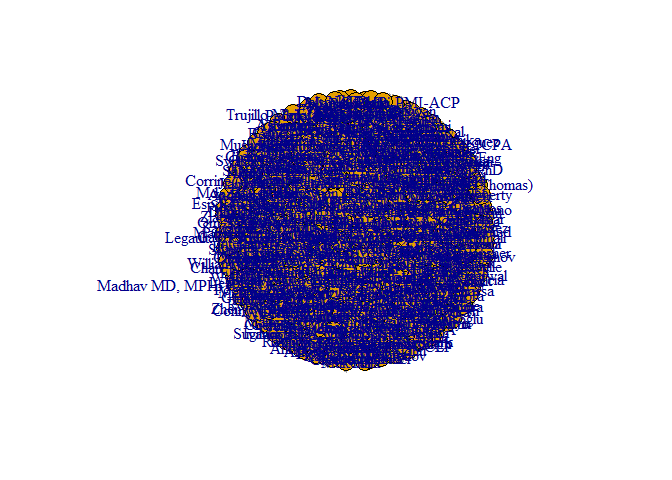
\includegraphics{Exercise_1_files/figure-latex/Step 5.2-1.pdf} Note:
Because of the issues with `nodes\_df' and `edges\_df', plot is
displayed incorrectly and looks very busy.

\end{document}
